\documentclass[10 ,titlepage, a4paper]{article}
    \usepackage{mystyle}
\usepackage{tikz}
\usetikzlibrary{decorations.pathmorphing} % indispensable !
\usetikzlibrary{positioning}
\usetikzlibrary{fit}
\usepackage{varwidth} % dans le préambule

\thispagestyle{fancy}
\title{Notes of introduction to information processing}
\author{Dario Marcone}
\date{Samedi 08 novembre 2025}

\begin{document}
\maketitle

\thispagestyle{empty}
\tableofcontents
\newpage

\section{Linear algebra in Dirac notation}
    \begin{tcolorbox}[vert]
        \begin{itemize}[left=10pt, label=\textbullet]
            \item A \important{Hilbert space} is a vector space on complex numbers with an inner product stucture. 
            \item $\mathcal{H},\mathspace dim\mathcal{H}=d, \mathspace \text{colon vectors: } \vec{\psi}=\begin{pmatrix} \psi_1 \\ \ldots \\ \psi_d \end{pmatrix}, \mathspace \psi \in \mathbb{C}$, line vectors: $\vec{\psi}^{T, *} = \left(\psi_1^*, \psi_2^*, \ldots, \psi_d^*\right)$, scalar product: $\vec{\phi}^{T, *}\cdot \vec{\psi}=\sum_{ i=1 } ^{ d } \phi_i^*\psi_i$. 

                \textit{(* means conjugate)}
        \end{itemize}
    \end{tcolorbox}
    \subsection{Dirac notation}
    Ket: $\vec{\psi} = \ket{\psi}$, Bra: $\vec{\psi}^{T, *} = \bra{\psi}$, $\implies$ braket: $\vec{\phi}^{T, *} \vec{\psi} = \braket{\phi|\psi}$.
    \subsection{Propreties of Dirac}
        \begin{itemize}[left=10pt, label=\textbullet]
            \item \textbf{Linearity:} $\left(\alpha^*\bra{\psi_1}+\beta^*\bra{\psi_2}\right)\ket{\phi}=\alpha^*\braket{\psi_1|\phi}+\beta^*\braket{\psi_2|\phi}$ .
            \item \textbf{Dirac conjugate:} $\left(\ket{\phi}\right)^{T, *}=\bra{\phi}$.
            \item \textbf{Skew symmetry:} $\braket{\phi|\psi}^* = \braket{\psi|\phi}$.
            \item \textbf{Norm:} $\left\|\psi\right\|=\sqrt{\braket{\psi|\psi}}$ with properties:
                \begin{enumerate}[left=10pt]
                    \item $\left\|\psi\right\|\geq 0, \left\|\psi\right\|=0 \leftrightarrow \ket{\psi}=0$,
                    \item $\left\|\psi_1\right\|-\left\|\psi_2\right\|\leq \left|\ket{\psi_1}+\ket{\psi_2}\right| \leq \left\|\psi_1\right\| + \left\|\psi_2\right\|$ ,
                    \item  $\left|\braket{\phi|\psi}\right| \leq \left\|\phi\right\|\cdot \left\|\psi\right\|$.
                \end{enumerate}
                
            \item \textbf{Basis:}
                \begin{enumerate}
                    \item Orthonormal Basis: $\{\ket{v_1}, \ket{v_2}, \ldots, \ket{v_d}\}$, then $\braket{v_i|v_j}=\begin{functionbypart}{\delta_{ij}}
                        1, \mathspace i = j  \\
                        0, \mathspace i \neq j
                    \end{functionbypart}.
                    $
                    \item Other basis: $\frac{\ket{0}+\ket{1}}{\sqrt{2}}=\frac{1}{\sqrt{2}}=\frac{1}{\sqrt{2}}\begin{pmatrix} 1 \\ 1 \end{pmatrix} \equiv \ket{+}, \mathspace \frac{\ket{0}-\ket{1}}{\sqrt{2}}=\frac{1}{\sqrt{2}}\begin{pmatrix} 1 \\ -1 \end{pmatrix} \equiv \ket{-}$.
                \end{enumerate}
                
                \item \textbf{Tensor product:} 

                   Linear:
                    $\left(\alpha\ket{0}+\beta\ket{1}\right)\otimes\left(\gamma\ket{0}+\delta\ket{1}\right)=\alpha \gamma\ket{0}\otimes\ket{0}+\alpha\delta\ket{0}\otimes\ket{1}+\beta \gamma\ket{1}\otimes\ket{0}+\beta\delta\ket{1}\otimes\ket{1}$.
                    \begin{remark}{Example}
                        \begin{tcolorbox}[rouge]
                            Let $\mathcal{H}=\mathbb{C}^2, \mathspace \ket{0}= \begin{pmatrix} 1 \\ 0 \end{pmatrix}, \ket{1}=\begin{pmatrix} 0 \\ 1 \end{pmatrix} $, then
                            \[\ket{0} \otimes \ket{0} = \ket{00} = \begin{pmatrix} 1 \\ 0 \\ 0 \\ 0 \end{pmatrix}, \mathspace \ket{0} \otimes \ket{1} = \ket{01}= \begin{pmatrix} 0 \\ 1 \\ 0 \\ 0 \end{pmatrix},\] 
                            \[\ket{1} \otimes \ket{0} = \ket{10}= \begin{pmatrix} 0 \\ 0 \\ 1 \\ 0 \end{pmatrix}, \mathspace \ket{1} \otimes \ket{1} = \ket{11} = \begin{pmatrix} 0 \\ 0 \\ 0 \\ 1 \end{pmatrix} .\]
                        \end{tcolorbox}
                    \end{remark}
                        
                    
            \item \textbf{Matrices:}
                \begin{itemize}[left=10pt, label=\textendash]
                    \item Dagger: $A^{T, *} = A^{\dagger}, \mathspace \left(A\ket{\psi}\right)^{T, *}=\left(A\ket{\psi}\right)^{\dagger} = \left(\ket{\psi}\right)^{\dagger}A^{\dagger}=\ket{\psi}A^{\dagger}$.
                    \item Notation: Let $\{\ket{v_1}, \ldots, \ket{v_3}\}$ an orthonormal basis and $A_{ij}=\bra{v_i}A\ket{v_j}$ ((i,j)th element of the matrice), then $A = \sum_{ i,j = 1 } ^{ d }A_{ij}\ket{v_i}\bra{v_j}$. 
                    \item Hermitian matrices: $A^{\dagger}=A$ (self-adjoint), i.e. $\begin{pmatrix} 1 & i  \\ -i &  0 \end{pmatrix}$. 
                    \item Unitary matrices: $U^{\dagger}U=UU^{\dagger}=\mathbbm{1}, \mathspace U^{\dagger}=U^{-1}$, with properties:
                        \begin{enumerate}[left=10pt]
                            \item $\left\|U\ket{\psi}\right\|=\left\|\ket{\psi}\right\|$,
                            \item $\left(\bra{\phi}U^{\dagger}\right)\left(U\ket{\psi}\right)=\braket{\phi|\psi}$.
                        \end{enumerate}
                \end{itemize}
        \end{itemize}
\section{5 principles of quantum mechanics}
    \subsection{State of a system}
        \begin{tcolorbox}[vert]
            The state of an \important{isolated} system is a vector $\ket{\phi} \in \mathcal{H}$ in Hilbert space $\mathcal{H}$ w.r.t the normalization condition $\braket{\phi|\phi}=1$.       
        \end{tcolorbox}
        \begin{remark}{Remarque}
            \begin{tcolorbox}[gris]
                $\ket{\phi}$ and $e^{i\lambda}\ket{\phi}, \lambda \in \mathbb{R}$ are physically equivalent.
            \end{tcolorbox}
        \end{remark}
        \begin{remark}{Examples}
           \begin{tcolorbox}[rouge]
              \begin{enumerate}[left=10pt]
                  \item  Let $\mathcal{H}=\mathbb{C}^2=\{\begin{pmatrix} \alpha \\ \beta \end{pmatrix} | \mathspace\alpha,\beta \in \mathbb{C}\}$ (qubit space), then
                  $\mathbb{C} \implies \ket{\psi}=\alpha\ket{0}+\beta\ket{1}, \mathspace \left|\alpha\right|^2+\left|\beta\right|^2=1=\alpha\alpha^*+\beta\beta^*$,
                  \item Physical system: Mach-Zehnder interferometer 
                  \item Let $\mathcal{H}=\mathbb{C}^d, \mathspace \begin{pmatrix} \alpha_1 \\ \ldots \\ \alpha_d \end{pmatrix} = \ket{\psi}=\sum_{ i = 1 } ^{ d }\alpha_i \ket{i}, \mathspace \sum_{ i=1 } ^{ d }\left(\alpha_i\right)^2=1,$ (qudit space).
              \end{enumerate}
               
           \end{tcolorbox}
        \end{remark}
    \subsection{States evolve with time}
        \begin{tcolorbox}[vert]
           As follows: $\left|\psi_t\right|= U_t\ket{\psi_0}$ where $U_t$ is unitary matrix.
        \end{tcolorbox}
        \begin{remark}{Example}
            \begin{tcolorbox}[rouge]
                We can desribe the transformation of the state of a particle by a prefecting reflecting mirror ($\ket{H} \to \ket{V} \text{ and } \ket{V}\to\ket{H}$), by 
                \[U = \begin{pmatrix} 0 & 1 \\ 1 & 0 \end{pmatrix}, \mathspace \ket{H}=\begin{pmatrix} 1 \\ 0 \end{pmatrix}, \mathspace \ket{V}=\begin{pmatrix} 0 \\ 1 \end{pmatrix},\] 
                \[\implies U\left(\alpha\ket{H} + \beta\ket{V}\right)= \beta\ket{H}+\alpha\ket{V}.\]
            \end{tcolorbox}
        \end{remark}
    \subsection{Observable quantities}
        \begin{tcolorbox}[vert]
            Quantities that we measure: ``observables'' are given by Hermitian matrices of dimension $\mathcal{H} \cdot \mathcal{H}$
        \end{tcolorbox}
        \begin{remark}{Example}
            \begin{tcolorbox}[rouge]
                Observable for 1 qubit $\left(\mathbb{C}^2\right)$: 
                \[A=a\mathbbm{1}+bX+cY+dZ, \mathspace A = a^{\dagger} \implies a,b,c,d \in \mathbb{R}\]
                \[\mathbbm{1}=\begin{pmatrix} 1 & 0 \\ 0 & 1 \end{pmatrix}, X= \begin{pmatrix} 0 & 1 \\ 1 & 0 \end{pmatrix}, Y=\begin{pmatrix} 0 & -i \\ i & 0 \end{pmatrix}, Z = \begin{pmatrix} 1 & 0 \\ 0 & -i \end{pmatrix}.\]
            \end{tcolorbox}
        \end{remark}
        \hypertarget{princ4}{}
        \subsection{Measurement give probability outcome}
            \begin{tcolorbox}[vert]
                When observable A is measured, the outcome is a random eigenvalue of A, call it $\lambda_i, i = 1, \ldots, d = dim \mathcal{H}$, the original state before measure $\ket{\psi}$ becomes after measurement an output state $\ket{v_i}$ with eigenvalues corresponding to $\lambda_i$. The probability distributioin associated to the output $\lambda_i, \ket{v_i}$ is $prob\left(i\right)=\left|\braket{v_i|\psi}\right|^2 \leftarrow $ \textbf{BORN RULE}.
            \end{tcolorbox}
            \begin{itemize}[left=10pt, label=\textbullet]
                \item Results of the measurement are eigenvalues $\lambda_i$ of observable A, 
                \item Every eigenvalue is associated to an eigenvector $\ket{v_i}$, 
                \item If the system is in the original state $\ket{\psi}$, the probability to obtain $\lambda_i$ is \[P\left(\lambda_i\right)=\left|\braket{v_i|\psi}\right|^2,\]
                \item After the measurement, the state collapse on the eigenvector: $\ket{\psi} \to \ket{v_i}$.
            \end{itemize}
            \begin{theoreme}
                Spectral Theorem: 

                Let A be an hermitian matrice $A = A^{\dagger}$ and let $A\ket{v_i}= \lambda_i\ket{v_i}, i = 1, \ldots, d = dim\mathcal{H}$
                \begin{itemize}[left=10pt, label=\textbullet]
                    \item $\lambda_i \in \mathbb{R}$,
                    \item $\ket{v_1}, \ldots, \ket{v_d}$ form an orthogonal basis,
                \end{itemize}
                    \important{$ \implies A=\sum_{ i =1 } ^{ d }\lambda_i \ket{v_i}\bra{v_i}= \begin{pmatrix} \lambda_1 & \ldots & 0 \\  & \ldots &  \\ 0 & \ldots & \lambda_d \end{pmatrix} $}.
            \end{theoreme}
            \begin{itemize}[left=10pt, label=\textbullet]
                \item Lemma: $\sum_{ i=1 } ^{ d }\left|\braket{v_i|\psi}\right|^2=1$,  because $\left\|\psi\right\|=1$.
                \item Property: 
                    \begin{itemize}[left=10pt, label=\textendash]
                        \item $E\left(A\right)=\sum_{ i=1 } ^{ d }\lambda_i \left|\braket{v_i|\psi}\right|^2=\bra{\psi}A\ket{\psi}$
                        \item Var$\left(A\right)=\bra{\psi}A^2\ket{\psi}-\bra{\psi}A\ket{\psi}^2$
                    \end{itemize}
            \end{itemize}
        \subsection{Composite system and entanglement}
            \begin{tcolorbox}[vert]
                The composite system of $\mathcal{H}_A$ and $\mathcal{H}_B$ is equal to $\mathcal{H}_{A\cup B}= \mathcal{H}_A \otimes \mathcal{H}_B$.
            \end{tcolorbox}
            \begin{remark}{Remarque}
                \begin{tcolorbox}[gris]
                    $dim\left(\mathcal{H}_A \otimes \mathcal{H}_B\right)=\left(dim\mathcal{H}_A\right)\left(dim\mathcal{H}_B\right)$.
                \end{tcolorbox}
            \end{remark}
            \begin{remark}{Example}
                \begin{tcolorbox}[rouge]
                    $\mathcal{H}_A = \mathbb{C}^2, \mathspace \mathcal{H}_B=\mathbb{C}^2, \mathspace \begin{functionbypart}{\mathbb{C}^2 \otimes \mathbb{C}^2}
                        \ket{00} = \ket{0} \otimes \ket{0}  \\
                        \ket{01} = \ket{0} \otimes \ket{1}  \\
                        \ket{10} = \ket{1} \otimes \ket{0}  \\
                        \ket{11} = \ket{1} \otimes \ket{1}  
                    \end{functionbypart}
                    $ 
                \end{tcolorbox}
            \end{remark}
            \textbf{Product states:} $\ket{\psi}=\ket{\phi_A} \otimes \ket{\chi_B}, \mathspace \psi \in \mathcal{H}_A \otimes \mathcal{H}_B,  \mathspace \phi \in \mathcal{H}_A, \mathspace \chi \in \mathcal{H}_B$.
            \begin{tcolorbox}[vert]
                Entangled states: $\nexists$ a factorisation of the state.
            \end{tcolorbox}
            \begin{remark}{Example}
                \begin{tcolorbox}[rouge]
                    
                    $\ket{\psi}=\frac{1}{\sqrt{2}}\left(\ket{0}\otimes\ket{0}+\ket{1}\otimes \ket{1}\right) \neq \left(\alpha\ket{0}+\beta\ket{1}\right)\otimes\left(\gamma\ket{0}+\delta\ket{1}\right)$.
                \end{tcolorbox}
            \end{remark}
            \begin{remark}{Apparté}
                \textbf{Bloch sphere of a qubit state vector:}

                $\ket{\psi}=\alpha\ket{0}+\beta\ket{1} = \cos\left(\frac{\theta}{2}\right)\ket{0} + e^{i\phi}\sin\left(\frac{\theta}{2}\right)\ket{1}$.
            \end{remark}
\section{Applications of principles}
    \subsection{Mach-Zehnder interferometer}
       \includegraphics[width=5cm]{images/1.png}
       \begin{itemize}[left=10pt, label=\textbullet]
           \item \textbf{Space:} $\mathcal{H}=\mathbb{C}^2=\{\begin{pmatrix} \alpha \\ \beta \end{pmatrix}, \mathspace \alpha & \beta \in \mathbb{C}, \left|\alpha\right|^2+\left|\beta\right|^2=1\}$.
           \item \textbf{Basis:} $\begin{pmatrix} 1 \\ 0 \end{pmatrix} = \ket{H}, \mathspace \begin{pmatrix} 0 \\ 1 \end{pmatrix} = \ket{V}, \mathspace \alpha\ket{H}+\beta\ket{V}=\ket{\psi}$.
           \item \textbf{Beam splitter:} $U = \frac{1}{\sqrt{2}}\begin{pmatrix} 1 & 1 \\ 1 & -1 \end{pmatrix} \left(\text{ Hadamard matrix}\right)$.
           \item \textbf{State after the beam splitter: }$U\ket{H}= \frac{1}{\sqrt{2}}\left(\ket{H}+\ket{V}\right)$. \begin{remark}{Remarque}
                   \begin{tcolorbox}[gris]
                        It's a very srange state that is at the same time horizontal and vertical. If it wasn't a qubit, it would either be completely reflected or it would go through. 
                   \end{tcolorbox}
           \end{remark}
       \item \textbf{Perfect mirror: } $R = \begin{pmatrix} 0 & 1 \\ 1 & 0 \end{pmatrix}, \mathspace RR^{\dagger}=R^{\dagger}R=1 \left(\text{\important{important condition!}}\right), \mathspace R^{\dagger}=R \left(\text{coincidence}\right)$.
       \item \textbf{State after the perfect mirror: }$RU\ket{H}=\frac{1}{\sqrt{2}}\left(R\ket{H}+R\ket{V}\right)=\frac{1}{\sqrt{2}}\left(\ket{V}+\ket{H}\right)$.
       \item \textbf{State after the second beam splitter: }$URU\ket{H}=\frac{1}{\sqrt{2}}\left(U\ket{V}+U\ket{H}\right)$.
       \item \textbf{State before the detector: }$\psi_{\text{before detector}}=2\cdot \frac{1}{2}\ket{H}=\ket{H}$.
       \item \textbf{Measurement: } model with orthogonal basis of $\mathcal{H}=\mathbb{C}^2= \{\ket{H} \text{and} \ket{V}\}$:

           At the end of the interferometer, we measure state $\ket{H} \text{ or state } \ket{V}$, 

           if we measure $\ket{H} \implies$ clic in $D_1 \implies$ register +1,

           if we measure $\ket{V}\implies$ clic in $D_1 \implies$ register -1.

           By the Born rule : 
           \begin{align*} 
               prob\left(+1\right)=\left|\braket{H|\psi_{\text{before detector}}}\right|^2 &= 1 \\
               prob\left(-1\right)=\left|\braket{V|\psi_{\text{before detector}}}\right|^2 &= 0
           \end{align*}
           If we follow the \textit{\hyperlink{princ4}{$4^{\text{th}}$ principle}}, then we know that $\ket{H}$ and $\ket{V}$ are the eigenvectors of our observable and $\left(+1\right)$ and $\left(-1\right)$ are the eigenvalues of our observable.

           By spectral theorem, we define our observable: $\left(+1\right)\ket{H}\bra{H}+\left(-1\right)\ket{V}\bra{V}=\begin{pmatrix} +1 & 0 \\ 0 & -1 \end{pmatrix} = Z$.

           Expectated value of (Z): $\bra{\psi_{\text{before detector}}}Z\ket{\psi_{\text{before detector}}}=\bra{H}\{\left(+1\right)\ket{H}\bra{H}+\left(-1\right)\ket{V}\bra{V}\}\ket{H}=\left(+1\right)\braket{H|H}\braket{H|H}+\left(-1\right)\braket{H|V}\braket{H|V}=\left(+1\right)$.

           
           Var(Z): $\bra{\psi}Z^2\ket{\psi}-\bra{\psi}Z\ket{\psi}^2=0$.
       \end{itemize}
    \subsection{Photon polarization}
        \begin{itemize}[left=10pt, label=\textbullet]
            \item \textbf{Classical electro-magnetic waves: }
                \begin{align*}
                    \text{Linear polarization: } \vec{E} &\propto \vec{E}_0 \begin{pmatrix} \cos \theta \\ \sin \theta \\ 0 \end{pmatrix} e^{i \omega t} e^{i\frac{2\pi}{\lambda}z},\\
                    \text{Circular polarization: } \vec{E} &\propto \vec{E}_0 \begin{pmatrix} 1 \\ i \\ 0 \end{pmatrix} e^{i\omega t} e^{i\frac{2\pi}{\lambda}z}.
                \end{align*}
                \begin{remark}{Remarque}
                    \begin{tcolorbox}[gris]
                       The polarization of an electro-magnetic wave indicate how the electrique field oscillate in space and time (it shows the direction).
                    \end{tcolorbox}
                \end{remark}
            \item \textbf{Photon quantum particles: }Photon quantum particles that carry electro-magnetic energy have a polarization state:  
                
                $\text{Linear polarization state: } \ket{\theta}&=\cos \theta \ket{x}+\sin \theta \ket{y}, \mathspace
                 \ket{\theta_{\perp}} &= -\sin \theta \ket{x} + \cos \theta \ket{y}.$

                 Circular polarization state: $\ket{\circlearrowleft} = \frac{1}{\sqrt{2}}\left(\ket{x}+i\ket{y}\right)=\frac{1}{\sqrt{2}}\begin{pmatrix} 1 \\ i \end{pmatrix}, \mathspace \ket{\circlearrowright}= \frac{1}{\sqrt{2}}\left(\ket{x}-i\ket{y}\right)=\frac{1}{\sqrt{2}}\begin{pmatrix} 1 \\ -i \end{pmatrix}$.
            \begin{remark}{Remarque}
                \begin{tcolorbox}[gris]
                    A classical electro-magnetic wave can be viewed as a collective state of many photons, each having the same polarization state. This photon polarization state determine the direction and the form of oscillation of the electric field in the corresponding classical wave.
                \end{tcolorbox}
                
            \end{remark}
            
        \end{itemize}
\section{Quantum key distribution (QKD)}
    Classical protcols rely on some mathematicals problems believed to be hard, but one day, if there is some strong enough computer, the security wouldn't be assured. QKD rely on physics! So it doesn't have this problem, the disavantage is that you should have a quantum channel.
    \subsection{Key distribution}
        \begin{enumerate}[left=10pt]
            \item Suppose Alice wants to send $\vec{m}$. She encodes it as $\vec{m} \oplus \vec{x}=\vec{z}$.
            \item Bob receives $\vec{z}$. He adds $\vec{x} \implies \vec{z} \oplus \vec{x}= \left(\vec{m} \oplus \vec{x}\right) \oplus \vec{x}=\vec{m}\oplus\left(\vec{x}\oplus\vec{x}\right)=\vec{m}$.
        \end{enumerate}
    \subsection{BB84 protocol}
        For quantum key distribution protocols, we assume that:
        \begin{itemize}[left=10pt, label=\textbullet]
            \item A, B share a public classical channel that is not spoofable.
            \item A, B share a public quantum channel that is spoofable.
        \end{enumerate}
        \begin{tcolorbox}[vert]
            Setting: Alice has generated $\left(\vec{x} \in \{0, 1\}\right)$ and wants to share it with Bob.
            \begin{enumerate}[left=10pt]
                \item Alice encodes $\vec{x}$ as a quantum state of qubit.
                \item Bob decodes the q-state back into qbitstring.
                \item Public communication phase (through the classical channel).
                \item Generation of the common secret key + security check.
            \end{enumerate}
        \end{tcolorbox}
        
               \begin{enumerate}[left=10pt]
            \item \textbf{Step Encoding:}

            Alice encodes each $x \in \{0,1\}$ in a random basis (either X or Z basis):
            \begin{itemize}[left=10pt, label=\textbullet]
                \item Z basis: $\ket{0}, \ket{1}, Z=\begin{pmatrix} 1 & 0 \\ 0 & -1 \end{pmatrix} $
                \item X basis: $\ket{-}=\frac{\ket{0}-\ket{1}}{\sqrt{2}}, \ket{+}\frac{\ket{0}+\ket{1}}{\sqrt{2}}, X=\begin{pmatrix} 0 & 1 \\ 1 & 0 \end{pmatrix} $
            \end{itemize}
            \begin{center}
            \begin{tabular}{c|c}
                  \textbf{$x_1$}& \textbf{Z basis}\\  % ligne 1
                  \hline
                   0 & $\ket{0}$\\  % ligne 2
                    1 & $\ket{1}$ \\
                    \hline
                      & \textbf{X basis} \\
                      \hline
                    0 & $\ket{+}$ \\
                    1 & $\ket{-}$
            \end{tabular}
            \end{center}
            Let define H such that: $H\ket{0}=\ket{+}, \mathspace H\ket{1}=\ket{-}$.

            Alice sends $\ket{0}\ket{+}\ket{-}\ket{0}\ket{1}\ket{1}\ket{+}$, so she sends:
            \[\ket{\psi_{x_1}}=H^{ei}\ket{x_1} \text{ where ei $\sim$ Unif \{0,1\}} \implies \ket{\psi_{\vec{x}}}= \bigoplus_{j=1}^{m} H^{ei}\ket{x_j}.\]
            
            \item \textbf{Step Decoding:}

                Bob recieves $\ket{\psi_{\vec{x}}}=\bigoplus_{j=1}^{m} H^{ei}\ket{x_j}$, he chooses a random basis to measure it. If Bob know the basis, he can decode easily, he doesn't!
                \begin{itemize}[left=10pt, label=\textbullet]
                    \item Case 1: Bob measure in the same basis chosen by Alice $\to$ prob(decoding correctly)=1.
                    \item Case 2: Bob measures in the wrong basis $\to$ prob(decoding correctly)=$\frac{1}{2}$.
                \end{itemize}
                $\implies$ prob(decoding correctly)=$\frac{1}{2}\cdot 1 + \frac{1}{2}\cdot \frac{1}{2}=\frac{3}{4}$. 
                
            \item \textbf{Step Public communication: }
                
                Alice has $\vec{x}:$ original bitstring, $\vec{e}:$ original choice of basis.

                Bob has $\vec{y}:$ decoded bitstring, $\vec{f}:$ Bob's choice of basis.

                They publish over the classical channel their choice of $\vec{e}, \vec{f}$, and for each bit, if the base agree they keep the bit, otherwise they discard it. At the end, Alice has $\widetilde{x} \subset \vec{x}$ and Bob has $\widetilde{y} \subset \vec{y}$.
            \item \textbf{Step Security check: }

                Let $\widetilde{x}, \widetilde{y}$ be of length k. Alice and Bob pick a subset of k bits to ``sacrifice'' them: they exchange the bits over the public channel, 
                \begin{itemize}[left=10pt, label=\textbullet]
                    \item if they match, we can exclude that there is an eavesdropper,
                    \item otherwise we can conclude that there is an eavesdropper so we abort the protocol.     
                \end{itemize}
                \begin{remark}{Remarque}
                    \begin{tcolorbox}[gris]
                        When the eavesdropper look at a qubit on the quantum channel, he has to measure the qubit $\implies$ the state of the particle collapse. So if Alice and Bob have the same basis, but not the same bit, they can assume that an eavesdropper has intercepted and measured a qubit in the wrong basis, and then sent a modified state to Bob.
                    \end{tcolorbox}
                \end{remark}
        \end{enumerate}
        Let now see what is the probability that Alice and Bob have the same bit knowing that an eavesdropper (Eve) intercept it.
        
        \[
        \begin{functionbypart}{\text{prob(Eve's measured bit agrees)}}
            \text{case 1: correct base} \implies \text{prob(correct)}=1 \\
            \text{case 2: wrong base}\implies \text{prob(correct)}=\frac{1}{2}
        \end{functionbypart}
      \]
            $\implies \text{prob(Eve's measured bit agrees)}=\frac{3}{4}$. 
            \[\begin{functionbypart}{\text{prob(Bob correct | Eve's intercepted)}}
                \text{case 1: Eve was correct} \implies \frac{3}{4}\cdot \frac{3}{4}=\frac{9}{16} \\
                \text{case 2: Eve was wrong} \implies \frac{1}{4}\cdot \frac{1}{2}\cdot \frac{1}{2}=\frac{1}{16}
            \end{functionbypart}
            \]
            $\implies$ prob(Bob correct | Eve intercepted)$=\frac{9}{16}+\frac{1}{16}=\frac{5}{8}$.
            \vspace{15pt}
            
            Maybe sometimes bits of Alice and Bob can disagree not because of an eavesdropper but because of \important{noise}! To deal with noise we can use some classical error connection.
      \begin{remark}{Example}
         \begin{tcolorbox}[rouge]
            \textbf{Repetition code:} Suppose noise flips with probability $\frac{1}{3}$. If i want to send a bit b over a noisy channel instead i'll send $bb\bar{b}$.
            \begin{itemize}[left=10pt, label=\textbullet]
                \item Binary linear code: $C \subset \mathbb{F}_2^m, \mathspace \left|C\right|=2^k, \left[m,k,d\right]$ with 
                   \begin{itemize}[left=10pt, label=\textendash]
                       \item m: length of the codeword,
                       \item k: actual # of bits of information per codeword, 
                       \item d: minimum distance of the code (minimum number of bits differing between 2 vectors in C, in general d=m).
                   \end{itemize}
            \end{itemize}
         \end{tcolorbox}
      \end{remark}
      In the BB84 protocol, we can apply this by supposing that we expect $\epsilon$ fraction of bits to differ between $\widetilde{x}$ and $\widetilde{y}$ because of noise. 
      \begin{itemize}[left=10pt, label=\textbullet]
          \item After step 3, Alice chooses an ECC C that corrects $\epsilon'$ fraction of the bits and compute $\vec{c}$ ($\epsilon' > \epsilon$).
          \item She sends $m=\widetilde{x}\oplus\vec{c}$ to Bob over the classical channel.
          \item Bob compute $\vec{c} \mathspace'=\widetilde{y}\oplus m=\left(\widetilde{x}\oplus\widetilde{y}\right)\oplus  \vec{c}$, where $\widetilde{x} \oplus \widetilde{y}=$ errors.
          \item Then because $\vec{c}\mathspace' = \vec{c} \oplus \text{errors}$, Bob can recover $\vec{c}$ with the ECC and compute $m \oplus \vec{c}= \left(\widetilde{x}\oplus\vec{c}\right)\oplus\vec{c}=\widetilde{x}$.
      \end{itemize}
\section{Entanglement}
    \hypertarget{defentro1}{}
    \begin{tcolorbox}[vert]
        Let be 2 parts: $A & B, \mathspace \mathcal{H}_{\text{total}}=\mathcal{H}_A \otimes \mathcal{H}_B$, then there is two types of states: 
        \begin{align*} 
            \text{\textbf{product states: }} &\ket{ \psi}=\ket{\phi_A}\otimes\ket{\chi_B}, \\
            \text{\textbf{entangled states: }} &\ket{\psi} \text{ such that } \nexists \text{ a factorization into tensor product. }
        \end{align*}
    \end{tcolorbox}
    \begin{remark}{Example}
        \begin{tcolorbox}[rouge]
            Let $\mathcal{H}_{\text{total}}=\mathbb{C}^2 \otimes \mathbb{C}^2, \mathspace \ket{\psi}=\alpha_{00}\ket{00}+\alpha_{01}\ket{01}+\alpha_{10}\ket{10}+\alpha_{11}\ket{11}, \mathspace \ket{ab}=\ket{a}\otimes\ket{b}, \mathspace a_{ij}\in\mathbb{C}, \mathspace\sum_{ i,j=\left(0,0\right) } ^{ \left(1,1\right) }\left|\alpha_{ij}\right|^2=1, \mathspace \braket{\psi|\psi}=1$.
            \textbf{Product state:} 
            
            \vspace{5pt}
            $\ket{\psi}=\left(\alpha\ket{0}+\beta\ket{1}\right)\otimes\left(\gamma\ket{0}+\delta\ket{1}\right)  $
            such that $\alpha_{00}=\alpha \gamma, \alpha_{01}= \alpha \delta, \alpha_{10}=\beta \gamma, \alpha_{11}= \beta \delta$.

            \vspace{5pt}
            det$\begin{pmatrix} \alpha_{00} & \alpha_{01} \\ \alpha_{10} & \alpha_{11} \end{pmatrix} = det\left(\alpha\right)_{ij}=\alpha_{00}\alpha_{11}-\alpha_{01}\alpha_{10}=\alpha \gamma \beta \delt=- \alpha \delta \beta \gamm=0$.

             $\ket{\psi}$ \important{ is a product state } $\iff$ det$\begin{pmatrix} \alpha_{00} & \alpha_{01} \\ \alpha_{10} & \alpha_{11} \end{pmatrix}=0$.
              \end{tcolorbox}
        
    \end{remark}     
    \begin{remark}{}
        \begin{tcolorbox}[rouge]
            \textbf{Entangled state: }


            We will use the Bell states: 
            \begin{itemize}[left=10pt, label=\textbullet]
                \item $\ket{B_{00}}=\frac{1}{\sqrt{2}}\left(\ket{00}+\ket{11}\right)$
                \item $\ket{B_{01}}=\frac{1}{\sqrt{2}}\left(\ket{01}+\ket{10}\right)$
                \item $\ket{B_{10}}=\frac{1}{\sqrt{2}}\left(\ket{00}-\ket{11}\right)$
                \item $\ket{B_{11}}=\frac{1}{\sqrt{2}}\left(\ket{01}-\ket{10}\right)$
            \end{itemize}
            Properties:
            \begin{enumerate}[left=10pt]
                \item They form an orthonormal basis of $\mathbb{C}^2 \otimes \mathbb{C}^2$
                \[\braket{B_{ij}|B_{ij}}=1, \mathspace \braket{B_{ij}|B_{kl}}, \mathspace \left(ij\right)\neq\left(kl\right).\]
                \item ``Rotation invariance'': $\ket{B_{00}}=\frac{1}{\sqrt{2}}\left(\ket{\theta}\otimes \ket{\theta}+\ket{\theta_{\perp}}\otimes \ket{\theta_{\perp}}\right) \forall \theta$.
            \end{enumerate}
        \end{tcolorbox}
    \end{remark}
    \subsection{Teleportation}
        \begin{tcolorbox}[vert]
            The goal of teleportation is to teleport a quantum state or some information from A to B without physically transporting any qubit, we will however send classical messages
        \end{tcolorbox}
        \begin{itemize}[left=10pt, label=\textbullet]
            \item \textbf{Initial situation: } 
            \[\overbrace{\mathbb{C}_1^2 \otimes \mathbb{C}_2^2}^{Alice} \otimes \overbrace{\mathbb{C}_3^2}^{Bob}, \mathspace \ket{\phi}_1=\alpha \ket{0}_1 + \beta \ket{1}_1, \mathspace \ket{B_{00}}_{23}=\frac{1}{\sqrt{2}}\left(\ket{00}+\ket{11}\right).\]
            
        \begin{center}
        \begin{tikzpicture}[scale=1.2, every node/.style={font=\small}]
            \node[circle, fill=black, inner sep=2pt, label=left:{$1$}] (A1) at (0,0) {};
            \node[circle, fill=black, inner sep=2pt, label=left:{$2$}] (A2) at (0,0.8) {};
            \node at (0, 1.5) {A};
            \node[circle, fill=black, inner sep=2pt, label=right:{$3$}] (B3) at (3,0.8) {};
            \node at (3, 1.5) {B};
            \node at (1.6, 1.25) {entangled pair $\ket{B_{00}}_{23}$}
            \draw[thin] (1.5,0.8) ellipse [x radius=1.65, y radius=0.3];
        \end{tikzpicture}
        \end{center}
        \item \textbf{Final situation: }
        \[\ket{B_{??}}_{12},\mathspace\ket{\phi}_3=\alpha \ket{0}_2+\beta\ket{1}_3.\]
        \begin{center}
        \begin{tikzpicture}[scale=1.2, every node/.style={font=\small}]
            \node[circle, fill=black, inner sep=2pt, label=left:{$1$}] (A1) at (0,0) {};
            \node[circle, fill=black, inner sep=2pt, label=left:{$2$}] (A2) at (0,0.8) {};
            \node at (0, 1.5) {A};
            \node[circle, fill=black, inner sep=2pt, label=right:{$3$}] (B3) at (3,0.8) {};
            \node at (3, 1.5) {B};
            \node at (1.6, 0.4) {entangled pair $\ket{B_{??}}_{23}$}
            \draw[thin] (0,0.4) ellipse [x radius=0.2, y radius=0.6];
        \end{tikzpicture}
        \end{center}
        \item \textbf{Protocol steps:}
                \begin{enumerate}[left=10pt]
                    \item Alice does a Bell basis measurement in her lab, so her qubits collapse into one of the fourth possible Bell states, the total state becomes 
                    \[\left(\ket{B_{ij}}_{12}\bra{B_{ij}}_{12} \otimes \mathbbm{1}_3\right)\ket{\phi}_1 \otimes \ket{B_{00}}_{23}=\ket{B_{ij}}_{12} \otimes \ket{\widetilde{\phi}}_3.\]
                    \item Alice sends two classical bits of information to Bob: 00, 01, 10, 11.
                    \item Bob receives a classical message $ij \in \{00, 01, 10, 11\}$ and does the following: 
                    \begin{align*} 
                        00 &\to \text{Bob applies } \mathbbm{1} \text{ on his qubit}, \\
                        01 &\to \text{Bob applies } X_3 = \begin{pmatrix} 0 & 1 \\ 1 & 0 \end{pmatrix} \text{ on his qubit}, \\
                        10 &\to \text{Bob applies } Z_3 = \begin{pmatrix} 1 & 0 \\ 0 & -1 \end{pmatrix} \text{ on his qubit}, \\
                        11 &\to \text{Bob applies } Z_3X_3 = \begin{pmatrix} 0 & 1 \\ -1 & 0 \end{pmatrix} \text{ on his qubit}, \\
                    \end{align*}
                \end{enumerate}
        \end{itemize}
    \subsection{Dense coding}
        \begin{tcolorbox}[vert]
            The goal is to send two classical bits from A to B of information by one use of quantum channel.
        \end{tcolorbox}
        \begin{center}
        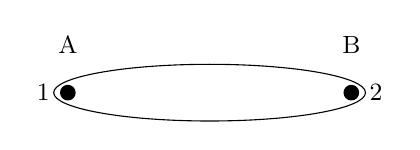
\begin{tikzpicture}[scale=1.2, every node/.style={font=\small}]
            \node[circle, fill=black, inner sep=2pt, label=left:{$1$}] (A1) at (0,0) {};
            \node at (0, 0.5) {A};
            \node[circle, fill=black, inner sep=2pt, label=right:{$2$}] (B2) at (3,0) {};
            \node at (3, 0.5) {B};
            \draw[thin] (1.5,0) ellipse [x radius=1.65, y radius=0.3];
        \end{tikzpicture}
        \end{center}
        \textbf{Protocol:}

            If Alice wants to encode 
            \begin{align*} 
                00 &\to \text{she applies } \mathbbm{1}_1 \otimes \mathbbm{1}_2 \ket{B_{00}}_{12}=\ket{B_{00}}_{12}, \\
                01 &\to \text{she applies } X_1 \otimes \mathbbm{1}_2 \ket{B_{00}}_{12}=\ket{B_{01}}_{12}, \\
                10 &\to \text{she applies } Z_1 \otimes \mathbbm{1}_2 \ket{B_{00}}_{12}=\ket{B_{10}}_{12}, \\
                11 &\to \text{she applies } Z_1X_1 \otimes \mathbbm{1}_2 \ket{B_{00}}_{12}=\ket{B_{11}}_{12}, \\
            \end{align*}
            Then she sends her obtained qubit so Bob have both qubit $\to$ the total state. So he knows which bits Alice encoded.
\section{Bell inequalities}
    \begin{tcolorbox}[vert]
        The goal here will be to ensure that A & B share an entangles Bell state (inequality) and as a consequence are able to produce common random secret strings of bits (Ekert 91 QKD protocol).
    \end{tcolorbox}
    Let
    \begin{center}
    \begin{tikzpicture}[scale=1.2, every node/.style={font=\small}]
        \node (A) at (0, 0.5) {A};
        \draw[->, , black, decorate, decoration={snake, amplitude=3pt, segment length=8pt}]
            (3.8,0) -- (0.1,0.5);
        \node (B) at (9, 0.5) {B};
        \draw[->, , black, decorate, decoration={snake, amplitude=3pt, segment length=8pt}]
            (5.2,0) -- (8.9,0.5);
        \draw[thin] (4.5,0) ellipse [x radius=0.65, y radius=0.3];

        \node at (4.5, 0) {source}
        \node[align=center] at (4.5, -1.0) {pairs of photons\\with pol. state. \\ $i=1, \ldots, N$.};

        \node[below=5pt of A,align=left] {
                \begin{varwidth}{4cm}
                measure the qubit.\\
            \begin{itemize}[left=0pt, label=\textbullet]
                \item basis: $\{\ket{\alpha}, \ket{\alpha_{\perp}}$,

                        record $a=\pm 1$.
                    \item basis \{$\ket{\alpha'}, \ket{\alpha_{\perp}'}$,\}

                        record $a'=\pm1$.
            \end{itemize}
            \end{varwidth}
            };
        \node[below=5pt of B,align=left] {
                \begin{varwidth}{4cm}
                measure the qubit.\\
            \begin{itemize}[left=0pt, label=\textbullet]
                \item basis: $\{\ket{\beta}, \ket{\beta_{\perp}}$,

                        record $b=\pm 1$.
                    \item basis \{$\ket{\beta'}, \ket{\beta_{\perp}'}$,\}

                        record $b'=\pm1$.
            \end{itemize}
            \end{varwidth}
            };
    \end{tikzpicture}
    \end{center}
    There is four possible measure settings for A and B: $1=\left(\alpha, \beta\right), 2=\left(\alpha', \beta\right), 3=\left(\alpha, \beta'\right), 4=\left(\alpha', \beta'\right)$.

    A and B meet or communcate classically and compute so-called correlation coefficient: 
    \[X_{exp}=\frac{1}{N_1}\sum_{ i_1 }a_i_1b_i_1+\frac{1}{N_2}\sum_{ i_2 }a_i_2'b_i_2+\frac{1}{N_3}\sum_{ i_3 }a_i_3b_i_3'+\frac{1}{N_4}\sum_{ i_4 }a_i_4'b_i_4'\]
    \newpage
    \noindent\textbf{Classical prediction $\left(X_{\text{class. th}}\right)$: }
    
    We assume a locality of measurement result, which means that $p_A\left(a\right)$ depends only of Alice's angle and $p_B\left(b\right)$ depends only of Bob's angle, 
    \[\implies p\left(a,b|\alpha,\beta,\lambda\right)=p_A\left(a|\alpha,\lambda\right)p_B\left(b|\beta,\lambda\right) \text{ with } \lambda = \text{ random variable with distribution }h\left(\lambda\right)d\lambda.\]
    \begin{tcolorbox}[violet]
        \textbf{Lemma:} 
         \[-2 \leq X_{\text{class. th.}} \leq 2 \text{ for } N \to +\infty.\]
    \end{tcolorbox}
    \noindent\textbf{Quantum theory:}
    \[X_{\text{th. quant.}}=\bra{B_{00}}A \otimes B \ket{B_{00}}+\bra{B_{00}}A' \otimes B \ket{B_{00}}-\bra{B_{00}}A \otimes B' \ket{B_{00}}+\bra{B_{00}}A' \otimes B' \ket{B_{00}}.\]
    Observables: 
    \[A= \left(+1\right)\ket{\alpha}\bra{\alpha}+\left(-1\right)\ket{\alpha_{\perp}}\bra{\alpha_{\perp}}, \mathspace B = \left(+1\right)\ket{\beta}\bra{\beta}+ \left(-1\right)\ket{\beta_{\perp}}\bra{\beta_{\perp}},
    \]
    \[
    \text{with }   \ket{\alpha}= \cos\alpha\ket{0}+\sin\alpha\ket{1}, \mathspace \ket{\alpha_{\perp}}= -\sin\alpha\ket{0}+\cos\alpha\ket{1} \text{ and same for }\beta.\]
    \[\implies X_{\text{th. quant.}}= \cos\left(2\left(\alpha-\beta\right)\right)+\cos\left(2\left(\alpha'-\beta\right)\right)-\cos\left(2\left(\alpha-\beta'\right)\right)+\cos\left(2\left(\alpha'-\beta'\right)\right).\]
    Entanglement induces non-locality, so according to QM:
\[p\left(a,b|\alpha,\beta\right)=\left|\braket{\text{state after meas.}|B_{00}}\right|^2=\frac{1}{4}\left(1+ab\cos\left(2\left(\alpha-\beta\right)\right)\right)\neq p_A\left(a|\alpha\right)p_B\left(b|\beta\right).
\]
    If we choose angles when $X_{\text{th. quant.}}$ is maximal $\left(\beta=\frac{\pi}{8}, \mathspace \alpha=0, \mathspace \beta'=-\frac{\pi}{8}, \mathspace \alpha'=-\frac{\pi}{8}\right)$, then $X_{\text{th. quant.}}= 2 \sqrt{2}$ \textbf{> 2! It violates the Lemma!}

    \vspace{5pt}
           \noindent If source distribute tensor product state $\ket{\phi_A} \otimes \ket{\phi_B} \in \mathbb{C}^2 \otimes \mathbb{C}^2$ then: 
           \[p\left(a,b|\alpha, \beta\right)=\left|\braket{\text{state after meas.}|\left(\ket{\phi_a}\otimes \ket{\phi_B}\right)}\right|^2\]
           \[= \underbrace{\left(\left(\frac{1+a}{2}\right)\left|\braket{\alpha|\phi_A}\right|^2\left(\frac{1-a}{2}\right)\left|\braket{\alpha_{\perp}|\phi_A}\right|^2\right)}_{p_A\left(a|\alpha\right)}\underbrace{\left(\left(\frac{1+b}{2}\right)\left|\braket{\beta|\phi_B}\right|^2\left(\frac{1-b}{2}\right)\left|\braket{\beta_{\perp}|\phi_B}\right|^2\right)}_{p_B\left(b|\beta\right)}.\]
           \begin{tcolorbox}[vert]
               If the pair is a product state it can't be greater than 2, $\implies$ if the result violates the Bell inequality it's an entangled state!
           \end{tcolorbox}
    \subsection{Ekert 91}
    Let
    \begin{center}
    \begin{tikzpicture}[scale=1.2, every node/.style={font=\small}]
        \node (A) at (0, 0.5) {A};
        \draw[->, , black, decorate, decoration={snake, amplitude=3pt, segment length=8pt}]
            (3.8,0) -- (0.1,0.5);
        \node (B) at (9, 0.5) {B};
        \draw[->, , black, decorate, decoration={snake, amplitude=3pt, segment length=8pt}]
            (5.2,0) -- (8.9,0.5);
        \draw[thin] (4.5,0) ellipse [x radius=0.65, y radius=0.3];

        \node at (4.5, 0) {source}
        \node[align=center] at (4.5, -1.0) {EPR pairs,\\ $\ket{B_{00}}$.};

        \node[below=5pt of A,align=left] {
            \begin{varwidth}{4cm}
                measure in possible basis:
            \begin{itemize}[left=0pt, label=\textbullet]
                \item $\alpha_1=-\frac{\pi}{4}$,
                \item $\alpha_2=-\frac{\pi}{8}$,
                \item $\alpha_3=0$,
            \end{itemize}
            \end{varwidth}
            };
        \node[below=5pt of B,align=left] {
                \begin{varwidth}{4cm}
            measure in possible basis:
            \begin{itemize}[left=0pt, label=\textbullet]
                \item $\beta_1=-\frac{\pi}{8}$
                \item $\beta_2=0$
                \item $\beta_3=\frac{\pi}{8}$
            \end{itemize}
            \end{varwidth}
            };
    \end{tikzpicture}
    \end{center}
    A and B exchange the basis choices at each $1, \ldots, N$ and compute $X_{\text{Bell}}$ using the bits among $\left(x_i, y_i\right)$ only those corresponding to CSHS basis choice, $\left|X_{Bell}\right| \approx 2\sqrt{2}$, otherwise there is an eavesdropper.

    \important{Common key} one time pad is given by $x_i$ and $y_i$ such that A and B choose the same basis, $\left(\alpha_3, \beta_2\right)$ or $\left(\alpha_2, \beta_1\right)$. In this case $x_i=y_i$.

\section{Density matrix}
    There is two situations where density matrix are useful: 
    \begin{enumerate}[left=10pt]
        \item Statistical mixtures.
        \item Physical systems that are not isolated. 
    \end{enumerate}
    \subsection{Statistical mixture}
        \begin{tcolorbox}[vert]
            A statistical mixture is a system of N degrees of freedom (quantum particles), where 
            \begin{align*} 
                \text{fraction } &p_1 \text{ of degree of freedom is in state } \ket{\phi_1}\in\mathcal{H}, \\
                \text{fraction } &p_2 \text{ of degree of freedom is in state } \ket{\phi_2}\in\mathcal{H}, \\
                                 &\ldots \\
                \text{fraction } &p_k \text{ of degree of freedom is in state } \ket{\phi_k}\in\mathcal{H},
            \end{align*} 
            \[0 \leq p_i \leq 1, \sum_{ i=1 } ^{ k }p_i=1.\]
        \end{tcolorbox}
        Convenient useful description is through the density matrix: $\rho= \sum_{ i=1 } ^{ k } p_i \ket{\phi_i}\bra{\phi_i}$
        \begin{remark}{Remarque}
            \begin{tcolorbox}[gris]
                Density matrix is a convex linear combination of projections: $\ket{\phi_i}\bra{\phi_i}= \pi_i, \mathspace \pi_i\ket{\psi}= \ket{\phi_i}\braket{\phi_i|\psi},\mathspace \pi_i^+ = \pi_i, \mathspace \pi_i ^2=\pi_i$.
            \end{tcolorbox}
        \end{remark}
        From a statistical mixture, we get a state $\ket{\phi_i}$ with probability $p_i$, then we measure $\ket{\phi_i}$, what's the expectation of A?
        \begin{remark}{Remarque}
            \begin{tcolorbox}[gris]
                \textbf{Cyclicity of Trace:} 
                \[Tr\left(AB\right)=Tr\left(BA\right), \mathspace Tr\left(ABC\right)=Tr\left(CAB\right)=Tr\left(BCA\right).\]
            \end{tcolorbox}
        \end{remark}
        Expectated value of A notated <A>: 
        \[\sum_{ i=1 } ^{ k }p_i\bra{\phi_i}A\ket{\phi_i} 
            = \sum_{ i=1 }^{ k}p_i Tr\left(A\ket{\phi_i}\bra{\phi_i}\right)
            = Tr \{\sum_{ i=1 } ^{ k }p_iA\ket{\phi_i}\bra{\phi_i}\}
            = TrA\left(\sum_{ i=1 } ^{ k }p_i\ket{\phi_i}\bra{\phi_i}\right)=Tr\left(A\rho\right).
        \]
       $<A> = Tr\left(A\rho\right)=Tr\left(\rho A\right), \mathspace \mathspace \mathspace Var\left(A\right)= <A^2>-<A>^2=Tr\left(A^2\rho\right)-\left(Tr\left(A\rho\right)\right)^2$. 
       \begin{theoreme}
           \begin{enumerate}[left=10pt]
               \item A density matrix satisfies $\rho^{\dagger}=\rho, \mathspace \rho \geq 0, \mathspace Tr\rho=1$.
               \item Vice-versa any matrix satisfying these 3 proposition is a density matrix.
           \end{enumerate}
       \end{theoreme}
    \subsection{Partial trace}
        M acts on $\mathcal{H}_1 \otimes \mathcal{H}_2$, orthonormal basis can be $\ket{v_i} \otimes \ket{w_j}$ with $i = 1 \ldots dim\mathcal{H}_1$ and $j = 1 \ldots dim \mathcal{H}_2$.
        \[M= \sum_{ ij; kl } M_{ij; kl} \left(\ket{v_i}\otimes \ket{w_j}\right)\left(\ket{v_k} \otimes \ket{w_l}\right), \mathspace \mathspace M_{ij;kl}=\left(\ket{v_i} \otimes \ket{w_j}\right)M\left(\ket{v_k} \otimes \ket{w_l}\right).\]
        Full trace: $TrM=\sum_{ ij }M_{ij;ij}$,   $\mathspace \mathspace \mathspace $ partial trace: $Tr_{\mathcal{H}_1}M=\sum_{ j;l } \left(\sum_{ i } M_{ij; il}\right)\overbrace{\ket{w_j}\bra{w_l}}^{dim\mathcal{H}_2 \cdot dim\mathcal{H}_2}$.

        \begin{remark}{Remarque}
            \begin{tcolorbox}[gris]
                You can vizualize this by thinking that M like a big matrice of size $\left(dim\mathcal{H}_1 dim\mathcal{H}_2\right) \cdot \left(dim\mathcal{H}_1 dim\mathcal{H}_2\right)$ and that the partial trace correspond to slice this matrice in blocs corresponding to $\mathcal{H}_1$ and compute the trace on these blocs.
            \end{tcolorbox}
        \end{remark}
        \textbf{Properties:}
        \begin{itemize}[left=10pt, label=\textbullet]
            \item $Tr_{\mathcal{H}_1}Tr_{\mathcal{H}_2}M=\overbrace{Tr_{\mathcal{H}_1  \mathcal{H}_2}}^{\text{full trace}}M=Tr_{\mathcal{H}_2}Tr_{\mathcal{H}_1}M$,
            \item In special case $A \otimes B$: 
            \[Tr_{\mathcal{H}_1}\left(A \otimes B\right)=\left(Tr_{\mathcal{H}_1}A\right)B, \mathspace \mathspace Tr_{\mathcal{H}_2}\left(A \otimes B\right)=A\left(Tr_{\mathcal{H}_2}B\right), \mathspace \mathspace Tr_{\text{full}}A \otimes B=\left(Tr_{\mathcal{H}_1}A\right)\left(Tr_{\mathcal{H}_2}B\right).\]
        \end{itemize}
    \subsection{Partial density matrix}
        \begin{tcolorbox}[vert]
            Let $\rho$ be a full system $\mathcal{H}_{\text{full}} = \mathcal{H}_A \otimes \mathcal{H}_B$, then the local description of system A is given by 
            \[Tr_{\mathcal{H}_B}\rho\equiv\rho_A.\]
        \end{tcolorbox}
        When you have a non-isolated system S, it means that the system interact with an environement E, and $\ket{\psi} \in \mathcal{H}_S \otimes \mathcal{H}_E, \mathspace \rho_{S\cup E}=\ket{\psi}\bra{\psi}$.
        Then to compute the state of the sub-system S, you have to compute 
        \[\rho_S=Tr_E\ket{\psi}\bra{\psi}.\]
        Therefore, the general state of a non-isolated systemn is a density matrix!

        \noindent\textbf{Computation:}
        \begin{enumerate}[left=10pt]
            \item Choose an orthonormal basis on B: $\{\ket{i_B}\}, \mathspace i_B \in \{0,1\}^{n_B}$.
            \item $\rho_A=\sum_{ i_B }\left(\mathbbm{1}_A \otimes \bra{i_B}\right)\rho_{AB}\left(\mathbbm{1}_A \otimes \ket{i_B}\right)$.
        \end{enumerate}
        \textbf{Properties:}
        \begin{itemize}[left=10pt, label=\textbullet]
            \item If $M=A \otimes B$ thne $M_B = Tr\left(A\right)\cdot B$, 
            \item If $M$ a density matrix $= \rho_A \otimes \rho_B$ then $M_B= \underbrace{Tr\left(\rho_A\right)}_{=1}\rho_B=\rho_B$.
        \end{itemize}
\section{Von Neumann entropy}
    \subsection{Classical entropy}
        \begin{tcolorbox}[vert]
            For a random variable X, the entropy of X, $H\left(X\right) \approx $ amount of uncertainty: 
            \[H\left(X\right):= - \sum_{ i } p_i \log\left(p_i\right). \]
            $H\left(X\right)$ is maximized for the distribution over X that puts equal probabilities for all outcomes and is minimized if all its probability is on a single outcome.
        \end{tcolorbox}
    \subsection{Quantum entropy}
        \begin{tcolorbox}[vert]
            Let $\rho$ be a density matrix, its Von Neumann entropy is 
            \[S\left(\rho\right):= -Tr\left(\rho\log\left(\rho\right)\right).\]
        \end{tcolorbox}
        \begin{remark}{Remarque}
            \begin{tcolorbox}[gris]
                Diagonal elements of $\rho$ are a classical probability distribution, $Tr\left(\rho\log\rho\right)$ means:
                \begin{itemize}[left=10pt, label=\textbullet]
                    \item write $\rho$ in its eigenbasis: $\rho=\sum_{ i }\lambda_i \ket{i}\bra{i}$, 
                    \item $-Tr\left(\rho\log\rho\right)=-\sum_{ n = 1 } ^{ d }\lambda_i \log\left(\lambda_i\right)$.
                \end{itemize}
            \end{tcolorbox}
        \end{remark}
        \newpage
        \noindent\textbf{Properties:}
        \begin{itemize}[left=10pt, label=\textbullet]
            \item $S\left(\rho\right) \geq 0$, 
            \item $S\left(\rho\right)$ is maximal for $\rho= \frac{\mathbbm{1}}{d}= \begin{pmatrix} \frac{1}{d} & \ldots & 0 \\ \ldots &  \ldots & \ldots \\ 0 & \ldots & \frac{1}{d} \end{pmatrix} $, 
            \item $S\left(\rho\right)=0 \iff \rho$ is a pure state $\iff \rho = \ket{\psi}\bra{\psi}$, 
            \item Concavity: $S\left(\alpha\rho_1+\left(1-\alpha\right)\rho_2\right) \geq \alpha S\left(\rho_1\right) + \left(1-\alpha\right)S\left(\rho_2\right)$.
        \end{itemize}
    \subsection{Entropy of a single qubit}
        For a single qubit, the density matrix is 
        \[\rho=\frac{1}{2}\left(\mathbbm{1}+\vec{a}\cdot \vec{\sigma}\right)=\frac{1}{2}\begin{pmatrix} \mathbbm{1}+a_z & a_x+ia_y \\ a_x-ia_y & \mathbbm{1}-a_z \end{pmatrix} , \mathspace \mathspace \mathspace \mathspace\left\|\vec{a}\right\| <1, \mathspace \vec{\sigma}= \left[\sigma_x \mathspace \sigma_y \mathspace \sigma_z\right].\]
        Then we can do a basis change $\rho \to \rho'$ such that $S\left(\rho\right)=S\left(\rho'\right)$ but $S\left(\rho'\right)$ is much easier to calculate. For this case, the basis change is 
        \[\rho'=\begin{pmatrix} \frac{1+\left\|\vec{a}\right\|}{2} & 0 \\ 0 & \frac{1+\left\|\vec{a}\right\|}{2} \end{pmatrix} .\]
        because $\lambda_{1,2}=\frac{1 \pm \left\|\vec{a}\right\|}{2}$. 
        \[\implies S\left(\rho\right)=S\left(\rho'\right)=H\left(\frac{1+\left\|\vec{a}\right\|}{2}, \frac{1-\left\|\vec{a}\right\|}{2}\right).\]
    \subsection{Compute a partial density matrix}
        \begin{tcolorbox}[vert]
            If overall state $\in \mathcal{H}_{AB}$ is $\rho_{AB}$ with $n_A= #$qubits in A and $n_B = #$qubits in B, then  
            \begin{align*} 
                \rho_A &= \sum_{ i \in \{0,1\}^{n_B} } \left(I_A \otimes \bra{i}_B\right) \rho_{AB} \left(I_A\otimes \ket{i}_B\right), \\
                \rho_B &= \sum_{ i \in \{0,1\}^{n_A}} \left(\bra{i}_A \otimes I_B\right) \rho_{AB} \left(\ket{i}_A \otimes I_B\right).
            \end{align*}
        \end{tcolorbox}
        \textbf{Special case: $n_A = n_B=1$},  $\rho_{AB}=$
        
        \begin{center}
        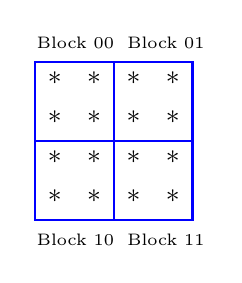
\begin{tikzpicture}
        \def\size{0.5} % taille d'une cellule
        \def\fs{6pt}     % taille de police pour les annotations
        
        % Dessin de la matrice 4x4 avec des *
        \foreach \i in {0,...,3} {
            \foreach \j in {0,...,3} {
            \node at (\j*\size, -\i*\size) {*} ;
            }
        }
        
        % Encadrement précis des blocs 2x2 (4 cellules par bloc)
        % Bloc haut-gauche (rouge)
        \draw[blue, thick]   (0-\size/2, 0+\size/2) rectangle (2*\size-0.5*\size, -2*\size+0.5*\size);
        % Bloc haut-droit (bleu)
        \draw[blue, thick]  (2*\size-0.5*\size, 0+\size/2) rectangle (4.5*\size-1*\size, -2*\size+0.5*\size);
        % Bloc bas-gauche (vert)
        \draw[blue, thick] (0-\size/2, -2*\size+0.5*\size) rectangle (2*\size-0.5*\size, -4*\size+0.5*\size);
        % Bloc bas-droit (orange)
        \draw[blue, thick](2*\size-0.5*\size, -2*\size+0.5*\size) rectangle (4.5*\size-1*\size, -4*\size+0.5*\size);
        \node[anchor=west, font=\fontsize{\fs}{\fs}\selectfont] at (-0.35, 0.5) {Block 00};
        \node[anchor=west, font=\fontsize{\fs}{\fs}\selectfont] at (\size + 0.3, 0.5) {Block 01};
        \node[anchor=west, font=\fontsize{\fs}{\fs}\selectfont] at (-0.35, -2) {Block 10};
        \node[anchor=west, font=\fontsize{\fs}{\fs}\selectfont] at (\size+0.3, -2) {Block 11};
        \end{tikzpicture} 
        \end{center}
        Then 
        \[\rho_A = \begin{pmatrix} * & * \\ * & * \end{pmatrix} = \begin{pmatrix} Tr\left(\text{Block 00}\right) & Tr\left(\text{Block 01}\right) \\ Tr\left(\text{Block 10}\right) & Tr\left(\text{Block 11}\right) \end{pmatrix} .\]
        This only works if we adopt the convention $ A \otimes B = \begin{pmatrix} A_{00}B & A_{01}B \\ A_{10}B & A_{11}B \end{pmatrix} $.
        \begin{remark}{Example}
            \begin{tcolorbox}[rouge]
               Let $\rho_{AB}=\ket{\psi_{Ab}}\bra{\psi_{AB}}$, where $\ket{\psi_{AB}}=\ket{0}_A \otimes \ket{+}_B$. Then 
               \[\rho_{AB}= \sigma_A \otimes \sigma_B \implies Tr_B\left(\rho_{AB}\right)=\sigma_A.\]
               Let's compute:
               \begin{align*} 
                   \ket{\psi_{AB}} &= \begin{pmatrix} 1 \\ 0 \end{pmatrix}_A  \otimes \frac{1}{\sqrt{2}}\begin{pmatrix} 1 \\ 1 \end{pmatrix}_B \\
                   \rho_{AB}&=\begin{pmatrix} 1 \\ 1 \\ 0 \\ 0 \end{pmatrix} \begin{pmatrix} 1 & 1 & 0 & 0 \end{pmatrix} \cdot \frac{1}{2} 
               \end{align*}
        \begin{center}
        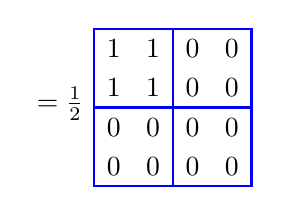
\begin{tikzpicture}
        \def\size{0.5} % taille d'une cellule
        \def\fs{6pt}     % taille de police pour les annotations
        
        % Dessin de la matrice 4x4 avec des *
        \foreach \i in {0,...,1} {
            \foreach \j in {0,...,1} {
            \node at (\j*\size, -\i*\size) {1} ;
            }
        }
        \foreach \i in {2,...,3} {
            \foreach \j in {2,...,3} {
            \node at (\j*\size, -\i*\size) {0} ;
            }
        }
        \foreach \i in {0,...,1} {
            \foreach \j in {2,...,3} {
            \node at (\j*\size, -\i*\size) {0} ;
            }
        }
        \foreach \i in {2,...,3} {
            \foreach \j in {0,...,1} {
            \node at (\j*\size, -\i*\size) {0} ;
            }
        }
        
        % Encadrement précis des blocs 2x2 (4 cellules par bloc)
        % Bloc haut-gauche (rouge)
        \draw[blue, thick]   (0-\size/2, 0+\size/2) rectangle (2*\size-0.5*\size, -2*\size+0.5*\size);
        % Bloc haut-droit (bleu)
        \draw[blue, thick]  (2*\size-0.5*\size, 0+\size/2) rectangle (4.5*\size-1*\size, -2*\size+0.5*\size);
        % Bloc bas-gauche (vert)
        \draw[blue, thick] (0-\size/2, -2*\size+0.5*\size) rectangle (2*\size-0.5*\size, -4*\size+0.5*\size);
        % Bloc bas-droit (orange)
        \draw[blue, thick](2*\size-0.5*\size, -2*\size+0.5*\size) rectangle (4.5*\size-1*\size, -4*\size+0.5*\size);
        \node[anchor=west] at (-1.1, -0.7) {$=\frac{1}{2}$};
        \end{tikzpicture} 
        \end{center}
                By doing the trace of each block: 
                \[\rho_A=\begin{pmatrix} 1 & 0 \\ 0 & 0 \end{pmatrix} =\ket{0}\bra{0}_A= \begin{pmatrix} 1 \\ 0 \end{pmatrix} \begin{pmatrix} 0 & 0 \end{pmatrix} .\]
                
 
            \end{tcolorbox}
        \end{remark}
    \subsection{Entanglement entropy}
        \begin{tcolorbox}[vert]
            Entanglement entropy answers the question: ``How much entanglement is in this quantum state?'', this is the von Neumann entropy of a reduced density matrix.
        \end{tcolorbox}
        We already know a definition of entanglement, but there is another one that use von Neumann entropy.
        \hypertarget{defentro2}{}
        \begin{tcolorbox}[vert]
            If you look at the reduced density matrix of a product state $\ket{\phi}_{AB}=\ket{\alpha}_A \otimes \ket{\beta}_B$ then you obtain $\rho_A=\ket{\alpha}\bra{\alpha}_A$ which is a pure state $\iff S\left(\rho_A\right)=0$.

            \vspace{5pt}
            So a general state $\ket{\psi}_{AB}$ is entangled $\iff S\left(\rho_A\right)\neq 0$.
        \end{tcolorbox}

        \begin{theoreme}
            If $\rho_A$ and $\rho_B$ come from a pure state, $S\left(\rho_A\right)=S\left(\rho_B\right)$.
        \end{theoreme}
        
        \begin{remark}{Examples}
            \begin{tcolorbox}[rouge]
                \begin{enumerate}[left=10pt]
                    \item \textbf{Product state:}
                    \[\ket{\psi}=\ket{\alpha}_A \otimes \ket{\phi}_B, \mathspace \mathspace \rho_A= \ket{\alpha}\bra{\alpha}_A, \mathspace \mathspace \rho_B=\ket{\phi}\bra{\phi}_B,\]
                    \[S\left(\rho_A\right)=S\left(\rho_B\right) \implies \text{theorem is correct.}\]
                    \item \textbf{Bell state:}

                        \noindent this state is famous being ``maximally entangled''. State on 2 qubits: 
                        \[\frac{1}{\sqrt{2}}\left(\ket{00}+\ket{11}\right), \text{ let's check if the definition hold:}\]
                        \[\rho_A=Tr_B\left(\ket{\psi}\bra{\psi}\right)=Tr\left(\frac{1}{2}\begin{pmatrix} 1 & 0 & 0 & 1 \\ 0 & 0 & 0 & 0 \\ 0 & 0 & 0 & 0 \\ 1 & 0 & 0 & 1 \end{pmatrix} \right)=\frac{1}{2}\begin{pmatrix} 1 & 0 \\ 0 & 1 \end{pmatrix} .\]
                        $\implies S\left(\rho_A\right)=1$, this Bell state is entangled, this is a maximally entangled state!
                \end{enumerate}
            \end{tcolorbox}
        \end{remark}
        \begin{remark}{Remarque}
            \begin{tcolorbox}[gris]
               A unique thing about quantum mechanics is that there existe some $\rho_{AB}$ such that $S\left(\rho_{AB}\right) < S\left(\rho_A\right)$. For example: $\rho_{AB}=\ket{B_{00}}\bra{B_{00}}$. 
            \end{tcolorbox}
        \end{remark}
        \begin{theoreme}
            \important{The Schmidt decomposition theorem} says that any state $\ket{\psi}_{AB}$ can be express as 
            \[\sum_{ i }p_i\ket{\phi_A}_i \otimes \ket{\phi_B}_i, \mathspace \mathspace p_i \geq 0.\]
            $\{\ket{\phi_A}_i\}$ is orthonormal for A and $\{\ket{\phi_B}_i\}$ is orthonormal for B, but they don't need to form a basis.
        \end{theoreme}
        \begin{remark}{Remarque}
            \begin{tcolorbox}[gris]
                If $r=1$, then $\ket{\phi}_{AB}$ is factorizable!
            \end{tcolorbox}
        \end{remark}
        
        Now, let's prove that : \hyperlink{defentro1}{\textit{first definition of entanglement}} $\iff$ \hyperlink{defentro2}{\textit{second definition of entropy}}.
        \begin{itemize}[left=10pt, label=\textbullet]
            \item \textbf{Definition 1 $ \implies $ definition 2:} 

                If $\ket{\psi}_{AB}$ can be factorized, then $S\left(\rho_A\right)$. So by contraposition, definition 1 $ \implies $ definition 2. 
                \item \textbf{Definition 2 $\implies$ definition 1:}

                    We can reformulize: if $\nexists$ a factorization then $S\left(\rho\right) > 0$. 

                    So by the Schmidt theorem, we can assume that: if $\nexists$ a way to write $\ket{AB}_{AB}= \ket{\phi}_A \otimes \ket{\sigma}_B \implies r > 1$. So $\ket{\psi}_{AB}= p_1\ket{\phi_1}_A \otimes \ket{\phi_1}_B+p_2\ket{\phi_2}_A\otimes \ket{\phi_2}_B+\ldots$

                    Then $p_1 > 0, \mathspace p_2 > 0 \implies \rho_A= p_1^2 \ket{\phi_1}\bra{\phi_1}+p_2\ket{\phi_2}\bra{\phi_2}+ \ldots$ because $\rho_A = \sum_{ i }\left(\mathbbm{1}_A \otimes \ket{\alpha_i}_B\right)\ket{\psi}\bra{\psi}_{AB}\left(\mathbbm{1}_A \otimes \ket{\alpha_i}_B\right)$ with $\{\ket{\alpha}_i\}\{\ket{\phi_B}_i\}$.

                    You can get then $\rho_A= \sum_{ i=1 } ^{ r }p_i^2\ket{\phi_i}\bra{\phi_i}_A, \mathspace \rho_B= \sum_{ i=1 } ^{ r }p_i^2\ket{\phi_i}\bra{\phi_i}_B$.

                    Then $S\left(\rho_A\right)= -\sum_{ i }p_i^2\log\left(p_i^2\right)=-p_1^2\log\left(p_1^2\right)-p_2^2\log\left(p_2^2\right)-\ldots > 0$.
        \end{itemize}
\section{Quantum error correction}
    Why do we use quantum error correction? Classical computers have some errors but quantum computers have much higher rates of errors (noise).
    \subsection{Classical error correction}
        One solution is \important{redundancy}: you encode n bits of information in m bits (m > n).
        \begin{remark}{Example}
            \begin{tcolorbox}[rouge]
                Let's suppose I want to send 1 bit over a noisy channel. 

                \textbf{Encoding:}
                \begin{align*} 
                    1 &\to 111 \\
                    0 &\to 000.
                \end{align*}
                Here $n =1$ and $m=3$.

                \textbf{Decoding:}
                
                Majority vote, $\bar{m}=abc \to $ output, whichevere bit is in the majority.
            \end{tcolorbox}
        \end{remark}
    \subsection{Model of quantum communication}
        \begin{center}
        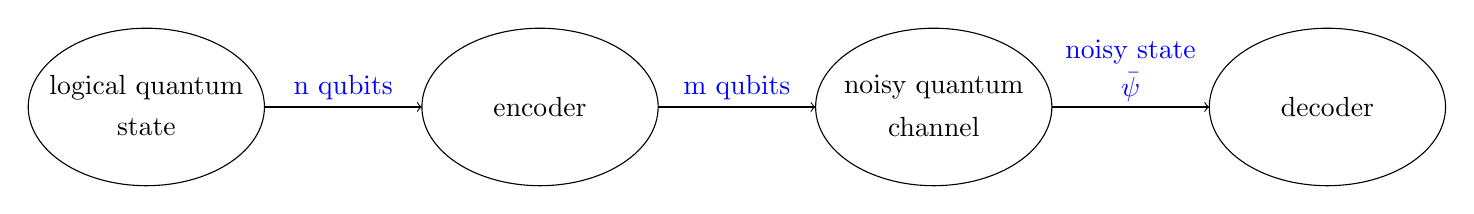
\begin{tikzpicture}
            \draw[thin] (-1,0) ellipse [x radius=1.5, y radius=1];
            \node at (-1, 0.25) {logical quantum};
            \node at (-1, -0.25) {state};
            \draw[thin] (4,0) ellipse [x radius=1.5, y radius=1];
            \node at (4, 0) {encoder};
            \draw[thin] (9,0) ellipse [x radius=1.5, y radius=1];
            \node at (9, 0.25) {noisy quantum};
            \node at (9, -0.25) {channel};
            \draw[thin] (14,0) ellipse [x radius=1.5, y radius=1];
            \node at (14, 0) {decoder};
            \draw[->, black] (0.5,0) -- (2.5,0);
            \node[blue] at (1.5, 0.25) {n qubits};
            \draw[->, black] (5.5,0) -- (7.5,0);
            \node[blue] at (6.5, 0.25) {m qubits};
            \draw[->, black] (10.5,0) -- (12.5,0);
            \node[blue] at (11.5, 0.7) {noisy state};
            \node[blue] at (11.5, 0.25) {$\ket{\bar{\psi}}$};
        \end{tikzpicture}
        \end{center}
    \subsection{Types of (single-qubit) quantum errors}
        \begin{itemize}[left=10pt, label=\textbullet]
            \item \textbf{X = bit flip error:} 
            \[X=\begin{pmatrix} 0 & 1 \\ 1 & 0 \end{pmatrix}, \mathspace \mathspace X\ket{0}=\ket{1}, \mathspace\mathspace X \ket{1}=\ket{0}, \mathspace\mathspace X\left(\alpha\ket{0}+\beta\ket{1}\right) = \alpha\ket{1}+\beta\ket{0}.\]
            
            \item \textbf{Z = phase flip error:}
                \[Z\ket{0}=\ket{0}, \mathspace\mathspace Z\ket{1}=-\ket{1}, \mathspace\mathspace Z\left(\alpha\ket{0}+\beta\ket{1}\right)=\alpha\ket{0}-\beta\ket{1}.\]
                \item \textbf{$R_{\theta}$ = Phase rotation:}
                    \[R_{\theta}=\begin{pmatrix} e^{-i\theta} & 0 \\ 0 & e^{i\theta} \end{pmatrix} .\]
        \end{itemize}
        \textbf{How des quantum error correction differ form classical error correction:}
        \begin{itemize}[left=10pt, label=\textbullet]
            \item  The no-cloning theorem forbids copying information. 
            \item We can't look at quantum states and figure out which copy is wrong.
            \item There are infinately many types of quantum errors. For example 
                \[R_{\theta}, \mathspace\mathspace \theta \sim \left[0,2\pi\left[  \mathspace\mathspace \to \text{ continuous}\]
                    \item We have Y errors on top of X and Z errors. Recall: 
                    \[X =\begin{pmatrix} 0 & 1 \\ 1 & 0 \end{pmatrix}, \mathspace \mathspace Y = \begin{pmatrix} 0 & -i \\ i & 0 \end{pmatrix}, \mathspaces \mathspace Z = \begin{pmatrix} 1 & 0 \\ 0 & -1 \end{pmatrix} .\]
        \end{itemize}


    \subsection{Detection and correction of bitflip errors}
        \textbf{Encoding:} Quantum repetition code 
        \begin{align*} 
            \ket{0} \mathspace &\to \mathspace \ket{000}, \\
            \ket{1} \mathspace &\to \mathspace \ket{000}, \\
            \ket{\psi} = \alpha\ket{0}+\beta\ket{1} \mathspace &\to \mathspace \alpha\ket{000}+ \beta\ket{111}.
        \end{align*}
        \begin{center}\includegraphics[width=5cm]{images/2.png} \end{center}
        \textbf{Decoding:} The idea is to check parity of every neibhouring pair
        \begin{center}\includegraphics[width=9cm]{images/3.png} \end{center}

        We assume that there was at most one error.
        \begin{center}
            \begin{tabular}{c|c|c}
                \textbf{a}& {\textbf{b}} & which qubit had error\\  % ligne 1
                  \hline
                0 & 0 & none \\  
                    \hline
                0 & 1  & 3 \\
                    \hline
                1 & 0 & 1  \\
                      \hline
                1 & 1 & 2
            \end{tabular}
            \end{center}
        But at the end, this QECC is not satisfying, because
        \begin{itemize}[left=10pt, label=\textbullet]
            \item It only handles one error out of 3 possible error locations. 
            \item You use 3 qubits to protect one 1 qubit (inefficient). 
            \item It only works for one type of error (bitflip).
        \end{itemize}
        To counter the third point, we will see phaseflip code a 9-qubit Shor code.
    \subsection{Detection and correction of phaseflip errors}
        The key fact in phaseflip detection and correction error is that phaseflip is a bitflip in a different basis.

        We already seen the effect of Pauli's matrices X and Z on base $\{\ket{0}; \ket{1}\}$, now let's see the effect on Hadamard basis $\{\ket{+}; \ket{-}\}$:
        \begin{itemize}[left=10pt, label=\textbullet]
            \item $X\ket{+} = X\left(\frac{\ket{0}+\ket{1}}{\sqrt{2}}\right)=\frac{\ket{1}+\ket{0}}{\sqrt{2}}=\ket{+}$, 
            \item $X\ket{-} = X\left(\frac{\ket{0}-\ket{1}}{\sqrt{2}}\right)=\frac{\ket{1}-\ket{0}}{\sqrt{2}}=-\ket{-}$, 
            \item $Z\ket{+} = Z\left(\frac{\ket{0}+\ket{1}}{\sqrt{2}}\right)=\frac{\ket{0}-\ket{1}}{\sqrt{2}}=\ket{-}$, 
            \item $Z\ket{-} = Z\left(\frac{\ket{0}-\ket{1}}{\sqrt{2}}\right)=\frac{\ket{0}+\ket{1}}{\sqrt{2}}=\ket{+}$, 
        \end{itemize}
        Phaseflip error is a bitflip error in Hadamard basis!
        \newpage
        \begin{tcolorbox}[vert]
            Let H be the change matrice between $\ket{0}\slash \ket{1}$ basis and $\ket{+} \slash \ket{-}$ basis, then 
            \begin{itemize}[left=10pt, label=\textbullet]
                \item $H\ket{0}=\ket{+}$, 
                \item $H\ket{1}=\ket{-}$, 
                \item $H\ket{+}=\ket{0}$, 
                \item $H\ket{-}=\ket{1}$,
                \item $HXH = Z$, 
                \item $HZH = X$.
            \end{itemize}
        \end{tcolorbox}
        \begin{center}
        \includegraphics[width=10cm]{images/4.png}
        \end{center}
        $\text{E}_{\text{phase}} =$ phase where phaseflip error occurs.   
        
       \noindent \textbf{Explanation:} The idea here is to apply bitflip encoding circuit, then change in Hadamard basis before the error phase, change in normal basis and apply bitflip decoding circuit.

       But what if we have both bitflip and phaseflip errors at the same time?
    \subsection{9-qubit Shor code}
        
        
        
           
        
        
\end{document}
